\subsection{Measuring thermal energy}

- The black body

	The theory of the black body is important to understand the absorbtion and emission of light relative to temperature, because the theory of the black body are used to describe the laws of infrared radiation and its relationship to temperature. The black body is an ideal perfect emitter of infrared radiation because it absorbs all electromagnetic radiation permitted to it, and it emits the same amount of radiation as it absorbs, the absorption and emission sums up to be zero. 
	Spectral emissive power, also denotted E_\lambda is the energy emitted by a surface in relation to time and range of wavelength. Figure \ref{fig:Spectral} shows an graphical illustration of spectral emissive power of the black body for specific wavelengths when the temperature changes. Radiation at different frequencies according to temperature are also shown in the figure. 
	
	The knowleadge of this principe helps in the understanding of how infrared radiation behaves, and how temperature affects the frequenzy of the signal. 
	
	The radiation from the human body which has a temperature at 37 degrees celcius emits the maximum energy of 9.3 \mu m, which means that most of the radiation is in the far infrared spectrum. Room temperature emits radiation higher in the infrared because the temperature is lower than the human body.
	
	- Maybe describe wien's displacement law... (wavelength of the peak of the blackbody radiation curve decreases as the body temperature increases)

	Stefan boltzmann's law? (radiation energy from black body is proportional ti the fourth power of its absolute temperature)
	
	Planck's law...
	
- RIO (region of interest)

	The lens are important to capture the image you want (dunno if this is relevant to mention?)

\begin{figure}[H]
	\centering	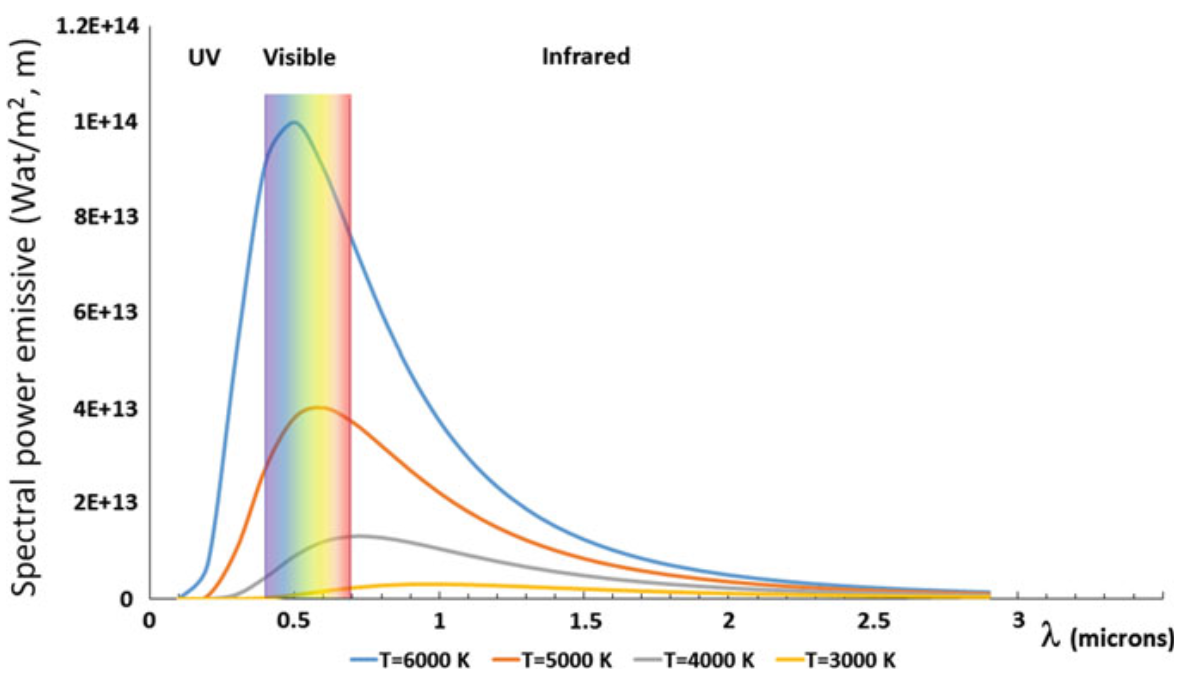
\includegraphics[width=0.65\textwidth]{figures/Spectral_power_emissive}
	\caption{Spectral power emissive}
	\label{fig:Spectral}
\end{figure} \vspace{-.3cm}

Measuring thermal radiation uses the knowledge that electromagnetic radiation is proportional to the internal energy. With a lens, the radiation that is emitted is focused onto a detector element in the camera that generates an electric output proportional to the radiation. The electric output is undergoing amplification and further signal processing.This allows the final output signal to be viewed as a temperature for the object. \cite{optris2009}
The black body is used for calibrating thermometers.

\begin{figure}[H]                                         
	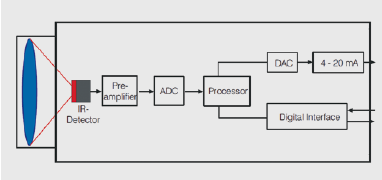
\includegraphics[width=.55\textwidth]{figures/IR_cam}  
	\caption{Simplified block diagram of an standard infrared camera.\cite{optris2009}}
	\label{fig:em_spectrum}  
\end{figure} 

extra notes that i'we just copied that we can use later 

The advantages of non-contact temperature measurement
are obvious – it supports:

• Temperature measurements of moving or overheated
objects and of objects in hazardous surroundings

• Very fast response and exposure times

• Non-interactive measurement, no influence on
the measuring object

• Non-destructive measurement

• Measurement point durability, no mechanical wear

